\documentclass[tikz,border=10pt]{standalone}
\usepackage{tikz}
\begin{document}
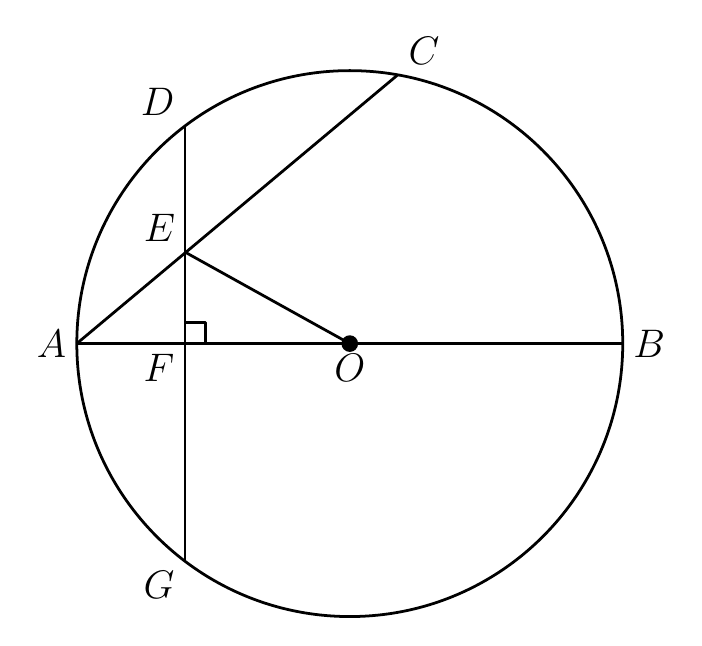
\begin{tikzpicture}[scale=0.017621, line width=1.0pt, line join=round]
  % Coordinates in pixels relative to O (y up), scaled by 0.017621 cm/px
  \coordinate (O) at (0,0);
  \coordinate (A) at (-196.7,0);
  \coordinate (B) at (196.7,0);
  \coordinate (F) at (-118.7,0);
  \coordinate (D) at (-118.7,156.9);
  \coordinate (G) at (-118.7,-156.7);
  \coordinate (C) at (34.7,193.7);
  \coordinate (E) at (-118.3,65.7);

  % Circle
  \draw (O) circle[radius=196.7];

  % Segments
  \draw (A) -- (B);
  \draw (D) -- (G);
  \draw (A) -- (C);
  \draw (O) -- (E);

  % Right-angle mark at F (sides along FB and FD, 15 px)
  \draw (-103.7,0) -- (-103.7,15) -- (-118.7,15);

  % Dot at O
  \fill (O) circle[radius=6];

  % Labels
  \node[font=\fontsize{14}{16.8}\selectfont, left] at (A) {$A$};
  \node[font=\fontsize{14}{16.8}\selectfont, right] at (B) {$B$};
  \node[font=\fontsize{14}{16.8}\selectfont, below] at (O) {$O$};
  \node[font=\fontsize{14}{16.8}\selectfont, below left] at (F) {$F$};
  \node[font=\fontsize{14}{16.8}\selectfont, above left] at (D) {$D$};
  \node[font=\fontsize{14}{16.8}\selectfont, below left] at (G) {$G$};
  \node[font=\fontsize{14}{16.8}\selectfont, above right] at (C) {$C$};
  \node[font=\fontsize{14}{16.8}\selectfont, above left] at (E) {$E$};
\end{tikzpicture}
\end{document}